\section{Database design}

\subsection{Misson}
Databasen har til formål at, hjælpe brugeren overskue hvilke droner han har til rådighed. Se hvilke status de har i systemet, om de er ude og flyve eller om de er i dock. Databasen trackker også hvilke events der forgår på nuværende tidspunkt og historik over events. Tilhørende events er information omkring flyve ruten, billeder tager på turen samt en log.

\subsection{Design}
På figuren \ref{fig:database_design} ses designet af databasen. Som beskrevet tidligere er database typen en SQLight database. Alt kommunikation til og fra databasen vil fungere igennem et database API. \\
Database API'et er et REST API som er udviklet ved brug af Django og Django REST frameworket. Ved kombinering af disse frameworks bliver databasen "pakket ind" og kan kun tilgås igennem API'et. Kommunikationen til og fra API'et forgå ved at sende/modtage JSON filer ved brug af API endpoints.

\subsubsection{Tilgængelige endpoints}
De tilgængelige endpoint i API'et er følgende:

\begin{table}[H]
\begin{tabular}{| p{3cm}| p{11.5cm}|}
\hline
Endpoint:	 							& \textbf{\textit{api/waypoints/}}\\\hline
Allows:									& POST, OPTIONS, GET\\\hline
Content-Type:						& application/json\\\hline 
Indehold:								& Giver adgang til waypoints tabellen, med muglighed for at tilføje nye waypoints\\\hline 
Kommentar:							& Det er muligt at tilføje "?format=json" til URL'en for at få dataen i ren json format\\\hline
\end{tabular}
\caption{Waypoint endpoint}
\label{waypoint_endpoint}
\end{table}

\begin{table}[H]
\begin{tabular}{| p{3cm}| p{11.5cm}|}
\hline
Endpoint:	 							& \textbf{\textit{api/users/}} \\\hline
Allows:									& OPTIONS, GET\\\hline
Content-Type:						& application/json\\\hline 
Indehold:								& Giver adgang til user tabellen\\\hline 
Kommentar:							& Det er muligt at tilføje "?format=json" til URL'en for at få dataen i ren json format\\\hline
\end{tabular}
\caption{User endpoint}
\label{user_endpoint}
\end{table}

\begin{table}[H]
\begin{tabular}{| p{3cm}| p{11.5cm}|}
\hline
Endpoint:	 							&\textbf{\textit{api/pictures/}} \\\hline
Allows:									& POST, OPTIONS, GET\\\hline
Content-Type:						& application/json\\\hline 
Indehold:								& Giver adgang til pictures tabellen, med mulighed for at tilføje nye billeder\\\hline 
Kommentar:							& Det er muligt at tilføje "?format=json" til URL'en for at få dataen i ren json format\\\hline
\end{tabular}
\caption{Picture endpoint}
\label{picture_endpoint}
\end{table}

\begin{table}[H]
\begin{tabular}{| p{3cm}| p{11.5cm}|}
\hline
Endpoint:	 							&\textbf{\textit{api/events/}}\\\hline
Allows:									& POST, PUT, OPTIONS, GET\\\hline
Content-Type:						& application/json\\\hline 
Indehold:								& Giver adgang til event tabellen, med mulighed for at oprette nye events og opdatere dem\\\hline 
Kommentar:							& Det er muligt at tilføje "?format=json" til URL'en for at få dataen i ren json format\\\hline
\end{tabular}
\caption{Event endpoint}
\label{event_endpoint}
\end{table}

\begin{table}[H]
\begin{tabular}{| p{3cm}| p{11.5cm}|}
\hline
Endpoint:	 							&\textbf{\textit{api/drones/}}\\\hline
Allows:									& POST, OPTIONS, GET\\\hline
Content-Type:						& application/json\\\hline 
Indehold:								& Giver adgang til drone tabellen, med mulighed for at tilføje nye droner\\\hline 
Kommentar:							& Det er muligt at tilføje "?format=json" til URL'en for at få dataen i ren json format\\\hline
\end{tabular}
\caption{Drones endpoint}
\label{drones_endpoint}
\end{table}

\begin{table}[H]
\begin{tabular}{| p{3cm}| p{11.5cm}|}
\hline
Endpoint:	 							&\textbf{\textit{api/drones/\#/}}\\\hline
Allows:									& PUT, OPTIONS, GET\\\hline
Content-Type:						& application/json\\\hline 
Indehold:								& Giver adgang til en record i drone tabellen, med mulighed for at opdatere droner\\\hline 
Kommentar:							& Det er muligt at tilføje "?format=json" til URL'en for at få dataen i ren json format\\\hline
\end{tabular}
\caption{Single drone endpoint}
\label{single_drone_endpoint}
\end{table}

\vspace{-5pt}
\begin{figure}[H]
	\centering
	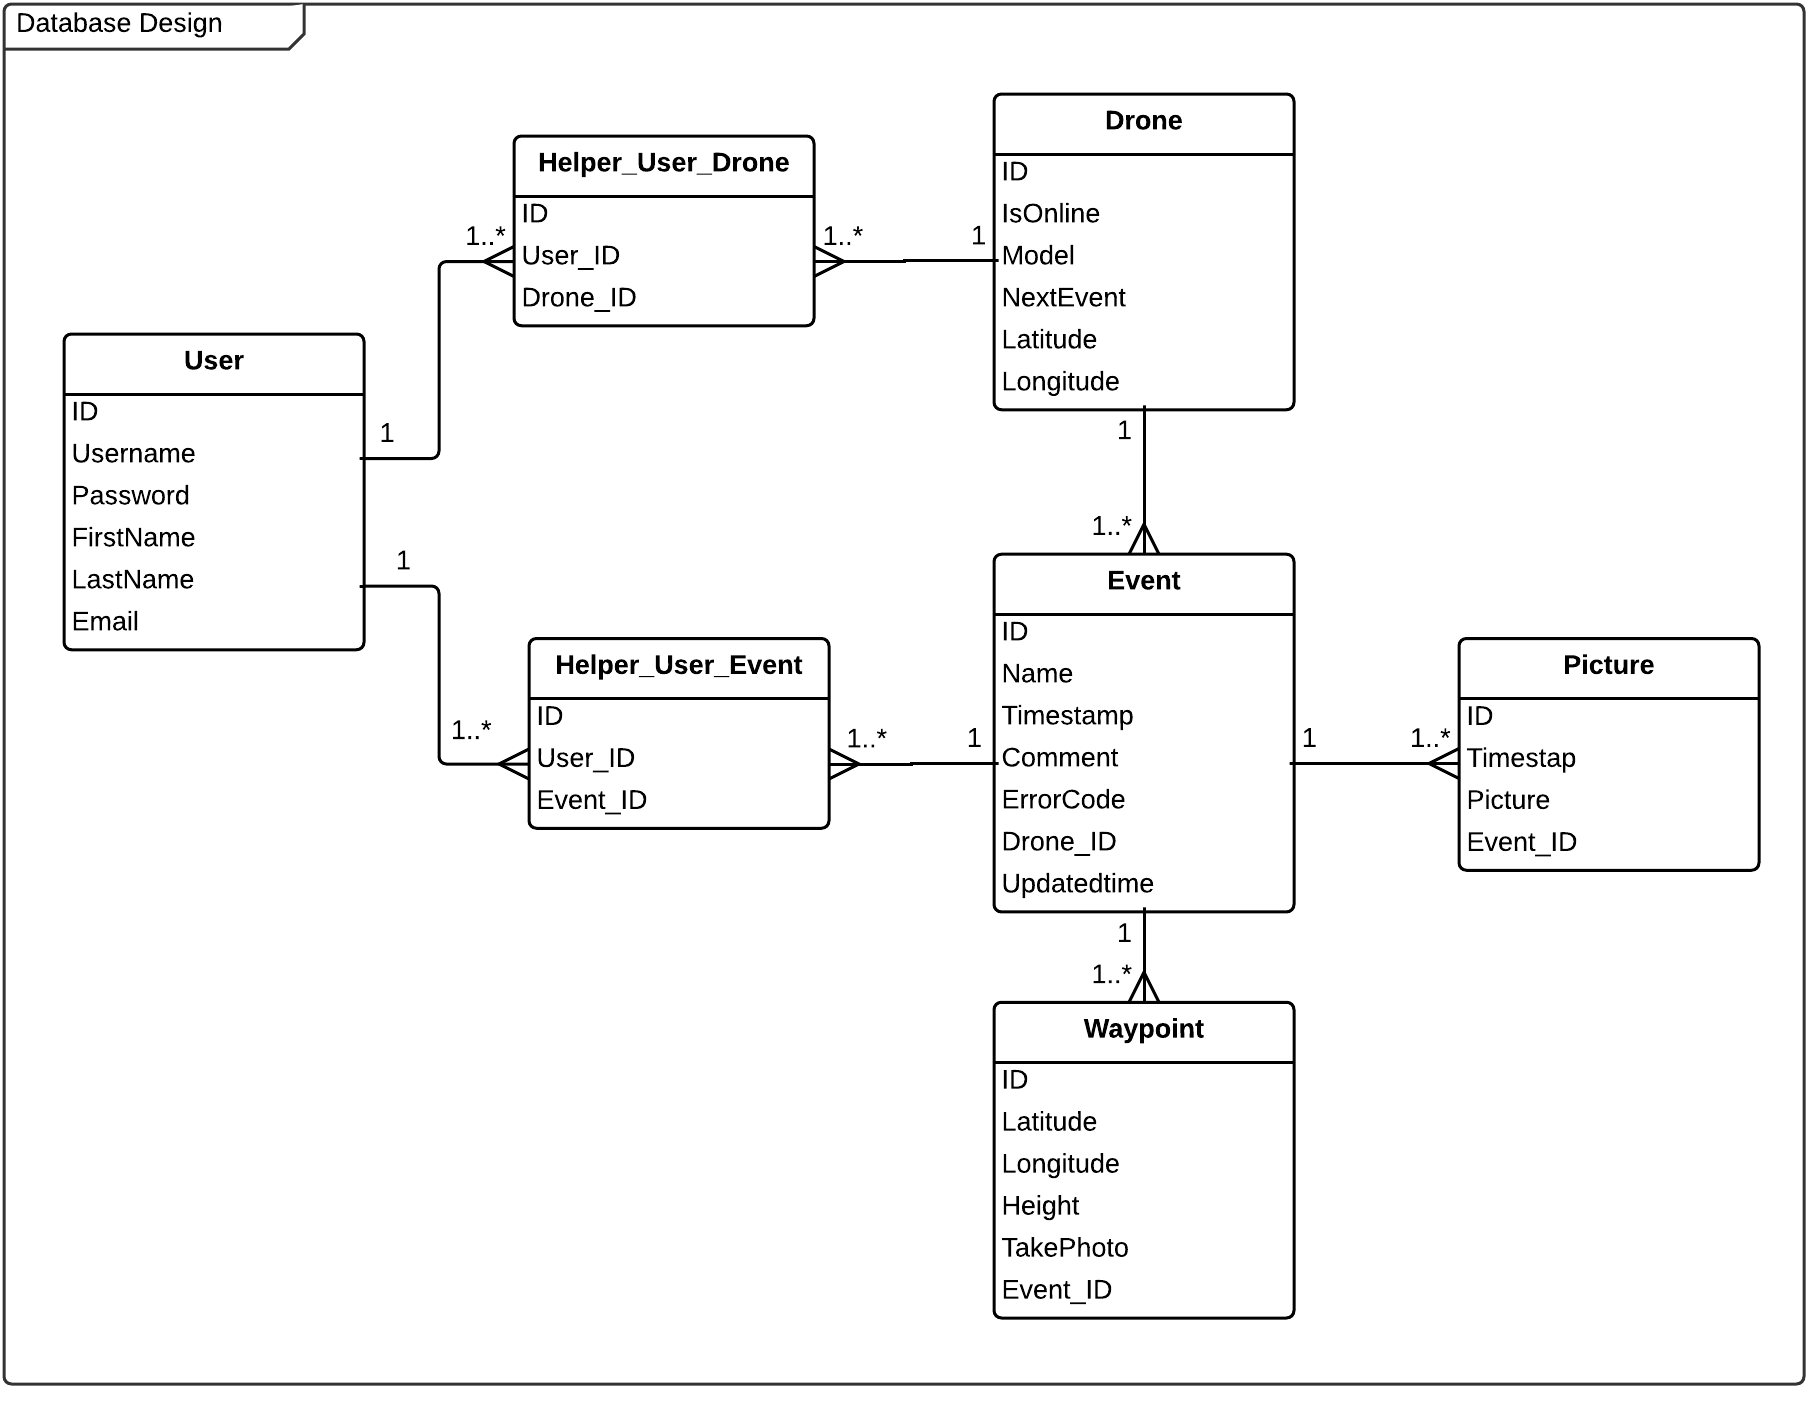
\includegraphics[width=1\textwidth]{Billeder/database/database_design.png}
	\vspace{-5pt}
	\caption{Database design}
	\label{fig:database_design}
\end{figure}

\newpage
\subsection{Database detaljeret beskrivelse}

\subsubsection{User table}
Tabellen indeholder data om den givet bruger i systemet. Tabellen giver også mulighed for brugeren at tilgå dronerne, events og de gemte ruter i systemet, via tabellens Foring keys.
\vspace{-5pt}
\begin{figure}[H]
	\centering
	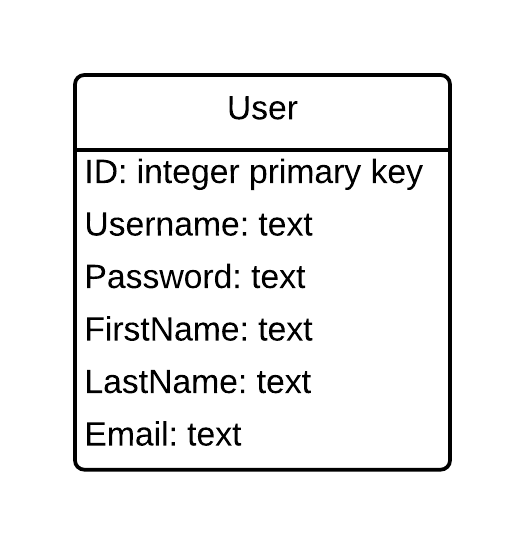
\includegraphics[width=0.5\textwidth]{Billeder/database/UserTabel.png}
	\vspace{-5pt}
	\caption{User table}
	\label{fig:user_table}
\end{figure}

\begin{table}[H]
\begin{tabular}{| p{3cm}| p{11.5cm}|}
\hline

Formål	 							& Holde data om brugeren i systemet, samt tjekke om brugeren eksterre ved forsøg på login.\\\hline
Forbindelser						& Tabellen har tre Foring keys til Helper User Drone og Helper User Event hjælpe tabellerne.\\\hline
Attributter						& \begin{itemize}
												\item ID: Primary key. Max length: 50 char
												\item Username: Brugernavnet til systemet. Max length: 50 char
												\item Password: Brugerens kode. Max length: 50 char
												\item FirstName: Brugers fornavn. Max length: 50 char
												\item LastName: Brugerens efternavn. Max length: 50 char
												\item Email: Brugerens email adresse.
											\end{itemize} \\\hline 
\end{tabular}
\caption{User table}
\label{tab:user_table}
\end{table}
